\documentclass[11pt,a4paper,fleqn]{scrartcl}

\usepackage[utf8]{inputenc}
\usepackage[T1]{fontenc}
\usepackage[colorlinks=true, citecolor=blue, linkcolor=blue, filecolor=blue,urlcolor=blue]{hyperref}
\hypersetup{
	colorlinks   = true,
	citecolor    = gray
}
\usepackage{wrapfig}

\usepackage{caption}
\captionsetup{format=plain, indent=5pt, font=footnotesize, labelfont=bf}


\setkomafont{disposition}{\scshape\bfseries}

\usepackage{amsmath}
\usepackage{fontawesome}
\usepackage{amssymb}
\usepackage{amsfonts}
\usepackage{bbm}
\usepackage{mathtools}
\usepackage{epsfig}
\usepackage{grffile}
%\usepackage{times}
%\usepackage{babel}
\usepackage{tikz}
\usepackage{paralist}
\usepackage{color}
\usepackage[top=3cm, bottom=2.5cm, left=2.5cm, right=3cm]{geometry}
%\setlength{\mathindent}{1ex}

\usepackage{palatino}
\usepackage{mathpazo}
\setlength\parindent{0pt}

% PGF
\usepackage{pgfplots}
\pgfplotsset{
  compat=newest,
  every axis/.append style={small, minor tick num=3}
}

\usepackage{natbib}
%\usepackage[backend=biber,style=alphabetic,url=false,doi=false]{biblatex}
%\addbibresource{sheet01_biber.bib}
% \addbibresource{/home/coroa/papers/refs.bib}

\newcommand{\id}{\mathbbm{1}}
\newcommand{\NN}{{\mathbbm{N}}}
\newcommand{\ZZ}{{\mathbbm{Z}}}
\newcommand{\RR}{{\mathbbm{R}}}
\newcommand{\CC}{{\mathbbm{C}}}
\renewcommand{\vec}[1]{{\boldsymbol{#1}}}


\renewcommand{\i}{\mathrm{i}}

\newcommand{\expect}[1]{\langle\,#1\,\rangle}
\newcommand{\e}[1]{\ensuremath{\,\mathrm{#1}}}

\renewcommand{\O}{\mc{O}}
\newcommand{\veps}{\varepsilon}
\newcommand{\ud}[1]{\textup{d}#1\,}

\newcommand{\unclear}[1]{\color{green}#1}
\newcommand{\problem}[1]{\color{red}#1}

%=====================================================================
%=====================================================================
\begin{document}

\begin{flushright}
 \textbf{Energy System Modelling }\\
 {\small Karlsruhe Institute of Technology}\\
 {\small Institute for Automation and Applied Informatics}\\
 {\small Summer Term 2020}\\
\end{flushright}

 
 \vspace{-0.5em}
 \hrulefill
 \vspace{0.3em}

\begin{center}
 \textbf{\textsc{\Large Tutorial II: Network Theory and Power Flow}}\\
 \small Will be worked on in the exercise session on Friday, 5 June 2020.\\[1.5em]
\end{center}

\vspace{-0.5em}
\hrulefill
\vspace{0.8em}

%=====================================================================
\paragraph{Problem II.1 (programming) -- network theory basics \faGroup}~\\
%=====================================================================

\begin{wrapfigure}[10]{r}{0pt}
 \centering
 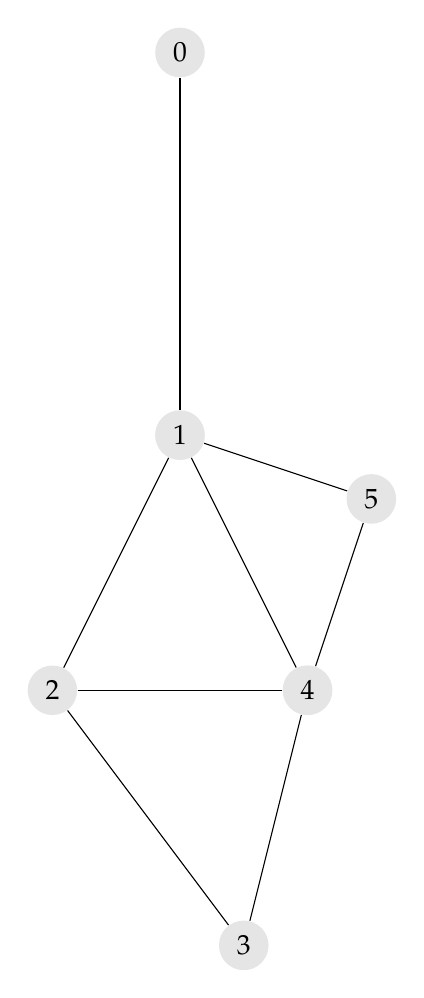
\begin{tikzpicture}
  [scale=.81,auto=left,every node/.style={circle,fill=gray!20}]
  \node (n0) at (2,14) {0};
  \node (n1) at (2,8)  {1};
  \node (n2) at (0,4)  {2};
  \node (n3) at (3,0) {3};
  \node (n4) at (4,4)  {4};
  \node (n5) at (5,7)  {5};
  \foreach \from/\to in {n0/n1,n1/n2,n1/n4,n1/n5,n2/n4,n2/n3,n3/n4,n4/n5}
  \draw (\from) -- (\to);
 \end{tikzpicture}
 \caption{Simple Network}
 \label{fig:network}
\end{wrapfigure}


Consider the simple network shown ins Figure \ref{fig:network}. Calculate in Python or by hand:

\begin{enumerate}[(a)]
 \item Compile the \textit{nodes list} and the \textit{edge list}.\\~\\
       \textbf{Remark:} While graph-theoretically both lists are unordered sets, let's agree on an ordering now which can serve as basis for the matrices in the following exercises: we sort everything in ascending numerical order, i.e.\ node 1 before node 2 and edge (1,2) before (1,4) before (2,3).
 \item Determine the \textit{order} and the \textit{size} of the network.
 \item Compute the\textit{ adjacency matrix} $A$ and check that it is symmetric.
 \item Find the \textit{degree} $k_n$ of each node $n$ and compute the \textit{average degree} of the network.
 \item Determine the \textit{incidence matrix} $K$ by assuming the links are always directed from smaller-numbered node to larger-numbered node, i.e.\ from node 2 to node 3, instead of from 3 to 2.
 \item Compute the \textit{Laplacian} $L$ of the network using $k_n$ and $A$. Remember that the Laplacian can also be computed as $L=KK^T$ and check that the two definitions agree.
 \item Find the \textit{diameter} of the network by looking at Figure \ref{fig:network}.

\end{enumerate}

\pagebreak
%=====================================================================
\paragraph{Problem II.2 (programming) -- linear power flow \faGroup}~\\
%=====================================================================



If you map the nodes to countries like \texttt{0=DK, 1=DE, 2=CH, 3=IT, 4=AT,5=CZ} the network in Figure \ref{fig:network2} represents a small part of the European electricity network (albeit very simplified). You can find the \textit{power imbalance} time series for the six countries for January 2017 in hourly MW in the file \texttt{imbalance.csv}. They have been derived from physical flows as published by ENTSO-E.\footnote{\url{https://transparency.entsoe.eu/transmission-domain/physicalFlow/show}}\\

The linear power flow is given by
\begin{equation}
 p_i = \sum_j \tilde{L}_{i,j}\theta_j \qquad \text{and} \qquad f_l = \frac{1}{x_l} \sum_i K_{i,l}\theta_i, \qquad \text{where} \qquad \tilde{L}_{i,j}= \sum_l K_{i,l}\frac{1}{x_l} K_{j,l}
\end{equation}
is the weighted Laplacian. For simplicity, we assume identity reactance on all links $x_l = 1$.

\begin{enumerate}[(a)]
 \item Compute the \textit{voltage angles }$\theta_j$ and \textit{flows} $f_l$ for the first hour in the dataset with the convention of $\theta_0 = 0$; i.e.\ the slack bus is at node 0.\\~\\
       \textbf{Remark:} Linear equation systems are solved efficiently using \texttt{numpy.linalg.solve}.
 \item Determine the average flow on each link for 01-2017 and draw it as a directed network.

\end{enumerate}

\begin{figure}[h]
 \centering
 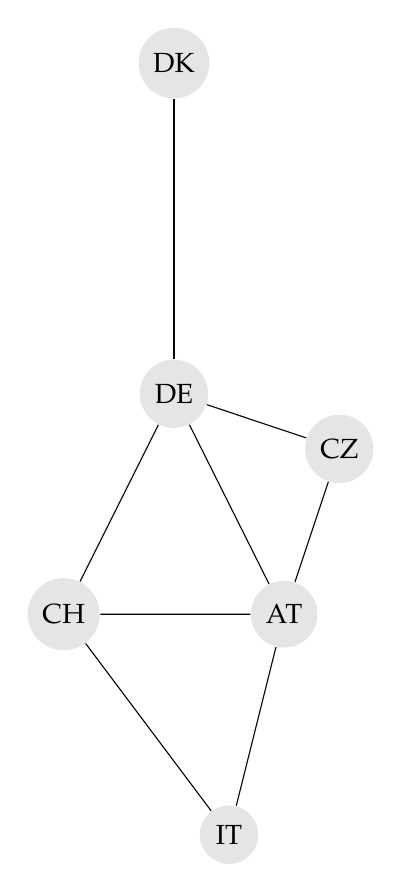
\begin{tikzpicture}
  [scale=.7,auto=left,every node/.style={circle,fill=gray!20}]
  \node (n0) at (2,14) {DK};
  \node (n1) at (2,8)  {DE};
  \node (n2) at (0,4)  {CH};
  \node (n3) at (3,0) {IT};
  \node (n4) at (4,4)  {AT};
  \node (n5) at (5,7)  {CZ};
  \foreach \from/\to in {n0/n1,n1/n2,n1/n4,n1/n5,n2/n4,n2/n3,n3/n4,n4/n5}
  \draw (\from) -- (\to);
 \end{tikzpicture}
 \caption{Simple Network}
 \label{fig:network2}
\end{figure}

%\bibliographystyle{unsrt}
%\bibliography{sheet02}
%\printbibliography

\end{document}
